% !TeX program = pdflatex
% Part IV of the godsil-gutman-lean series.
% When Walks Become a Spectrum — a machine-checked proof of Godsil's moment theorem
% p_k = treeLikeWalkCount in Lean 4.
% Build: pdflatex moment-theorem-lean.tex  (twice, for refs)

\documentclass[11pt]{article}
\usepackage[T1]{fontenc}
\usepackage{lmodern}
\usepackage{amsmath,amssymb,amsthm,booktabs,graphicx,hyperref}
\usepackage{xurl}
\usepackage[table]{xcolor}
\definecolor{ggteal}{HTML}{1B6F8C}
\definecolor{ggband}{HTML}{DCE7EB}
\definecolor{ggamber}{HTML}{E08A1E}
\usepackage[margin=1in]{geometry}
\usepackage{microtype}
\usepackage[most]{tcolorbox}
\usepackage{tikz}
\usetikzlibrary{arrows.meta,positioning,fit,backgrounds}
\setlength{\emergencystretch}{2em}
\newtheorem{theorem}{Theorem}
\newtheorem{lemma}{Lemma}
\newtheorem{definition}{Definition}
\newcommand{\lean}[1]{{\def\_{\textunderscore\allowbreak}\texttt{#1}}}
\newcommand{\Z}{\mathbb{Z}}
\newcommand{\R}{\mathbb{R}}
\newcommand{\C}{\mathbb{C}}
\newcommand{\N}{\mathbb{N}}
\DeclareMathOperator{\tr}{tr}
\DeclareMathOperator{\reflect}{reflect}
\DeclareMathOperator{\rev}{rev}
\DeclareMathOperator{\charpolyRev}{charpolyRev}
\providecommand{\llbracket}{[\![}
\providecommand{\rrbracket}{]\!]}
\hypersetup{colorlinks=true,linkcolor=ggteal,citecolor=ggteal,urlcolor=ggteal}
\newtcbox{\keybox}{on line,boxrule=0.9pt,colframe=ggteal,colback=ggband!40,
  arc=3pt,left=8pt,right=8pt,top=5pt,bottom=5pt}
\newcommand{\keyeq}[1]{\begin{center}\keybox{$\displaystyle #1$}\end{center}}
\newtcolorbox{classicalbox}[1][]{colframe=ggteal,colback=ggband!22,boxrule=0.9pt,arc=3pt,
  fonttitle=\bfseries,coltitle=white,colbacktitle=ggteal,title={#1},left=8pt,right=8pt,top=4pt,bottom=4pt}

\title{\bf When Walks Become a Spectrum\\[4pt]
  \large\normalfont A machine-checked proof of Godsil's moment theorem
  $p_k=\mathrm{treeLikeWalkCount}$ in Lean~4}
\author{Carles Mar\'in\thanks{Formalized with AI assistance (Claude, Anthropic); the mathematics
and all claims are the author's responsibility. The methodology is discussed in
Section~\ref{sec:methodology}.}\\[3pt]
  \normalsize Independent researcher\\
  \normalsize \texttt{karlesmarin@gmail.com}}
\date{June 2026}

\begin{document}
\maketitle

\begin{abstract}
This is the fourth piece of a series that builds, in Lean~4 / Mathlib, the two sides of the
matching/Ihara trace formula. In \emph{Walks that Forget the Cycles}~\cite{PartIII} I proved the
\emph{combinatorial} half of Godsil's moment theorem: the closed \emph{tree-like} walks of a graph
$G$ based at $v$ are in length-preserving bijection with the closed walks of Godsil's path tree
$T(G,v)$ based at its root, so that the tree-like walk count is a sum of adjacency-matrix powers,
$\mathrm{treeLikeWalkCount}(G,k)=\sum_v\bigl[A(T(G,v))^k\bigr]_{\mathrm{root}}$. That paper was
explicit about its boundary: the \emph{spectral} half---turning those matrix powers into the power
sums $p_k=\sum_i\theta_i^k$ of the roots of the matching polynomial $\mu(G)$---was \emph{mapped, not
built}. Here I build it, and close the theorem:
\[
  p_k(G)\;=\;\sum_i\theta_i^{\,k}\;=\;\mathrm{treeLikeWalkCount}(G,k),
  \qquad\text{machine-checked, \lean{sorry}-free.}
\]
The proof is a single power-series identity. On the trace side, each path tree's root--root resolvent
$\sum_k[A(T)^k]_{\mathrm{root}}X^k$ is, by a principal-minor determinant collapse, the ratio of two
reversed characteristic polynomials; Part~II's divisibility identity
$\mu(G)\mu(T-\mathrm{root})=\mu(G-v)\mu(T)$ rewrites it as a ratio of reversed \emph{matching}
polynomials; summing over $v$ and applying the vertex-deletion law $\sum_v\mu(G-v)=X\mu'(G)$ gives
$\mathrm{mk}(\mathrm{treeLikeWalkCount})\cdot\overline{\mu}=\overline{X\mu'}$. On the matching side, the
generating function of the root power sums equals, after a geometric-series cancellation against the
reversed factor product, the \emph{same} object $\overline{X\mu'}$. The two coincide; cancelling the
unit $\overline{\mu}$ and reading the coefficient of $X^k$ is the theorem. I record one honest
surprise: the completion needs \emph{no} univariate Newton identity---the route the prequel
predicted---only a reflection-at-fixed-degree bookkeeping of reversed polynomials. The headline
depends only on the three standard axioms; I am not aware of a prior formalization of Godsil's moment
theorem in any proof assistant. With this and the \emph{Bass} companion, both sides of the finite
trace formula now stand, \lean{sorry}-free, in one library.
\end{abstract}

\noindent\emph{Reader's map.} If you read only one thing, read Theorem~\ref{thm:moment} and the shape
of its proof: \emph{both} generating functions, the walk-counting one and the eigenvalue-power-sum
one, are forced to equal one and the same reversed polynomial $\overline{X\mu'(G)}$
(Figure~\ref{fig:weld}). Everything else is the careful version of that sentence---a per-vertex
identity that turns the trace side into reversed matching polynomials (Section~\ref{sec:trace}), a
geometric-series cancellation that turns the matching side into the same (Section~\ref{sec:match}),
and a coefficient-extraction once a unit is cancelled (Section~\ref{sec:weld}). The honest
surprise---no Newton---is Section~\ref{sec:boundary}; the limits and methodology,
Section~\ref{sec:methodology}; the next questions, Section~\ref{sec:questions}.

% ---------------------------------------------------------------
\section{Introduction: a count, and the spectrum it hides}
\label{sec:intro}

\emph{A graph's matching polynomial is not the characteristic polynomial of its adjacency matrix---so
where do the power sums of its roots live, and why are they a count of walks?} The prequel answered the first
clause with a tree and left the second as a promissory note; this paper redeems it. The route has a
long history---four centuries---and a small surprise waiting at its last step
(Section~\ref{sec:boundary}).

\paragraph{A thread, in five beads.} In 1629 Albert Girard wrote down what Newton would
systematize a generation later: the power sums $p_k=\sum_i\theta_i^k$ of a polynomial's roots are
fixed by its coefficients, and conversely, through a recursion now bearing Newton's
name~\cite{Girard,Macdonald}. That recursion is the canonical bridge between a polynomial's roots and
its data, and it will be the bead this paper, at its very end, declines to use. In 1972 Heilmann and
Lieb produced a polynomial that seemed to have no right to real roots at all---the matching
polynomial of a graph, born in the statistical mechanics of monomer--dimer systems---and proved its
roots real anyway~\cite{HeilmannLieb}, even though it is not the characteristic polynomial of the
graph's adjacency matrix unless the graph is a forest. In 1981 Godsil resolved the paradox with a single device, the
\emph{path tree}, and drew from it \emph{two} conclusions: that the matching polynomial is real-rooted
(it divides a forest's, and forests have symmetric spectra), and that its root power sums \emph{count
walks}~\cite{Godsil1981a,GodsilBook}. The fourth bead is the \emph{universal cover}: the path tree is
its finite truncation, the cover's spectral edge $2\sqrt{\Delta-1}$ is Godsil's bound on the matching
roots and the Ramanujan threshold~\cite{AngelFriedmanHoory,McKay,MSS}, and the walk count is a finite
shadow of a trace formula on the cover. The fifth bead is this series: Part~II carried Godsil's first
conclusion into Lean~\cite{PartII}, Part~III carried the combinatorial half of the
second~\cite{PartIII}, and this paper carries the rest---and, threading the last bead, comes back
unexpectedly to the first (Section~\ref{sec:boundary}).

\paragraph{The polynomial off the adjacency spectrum.} A finite graph $G$ on $n$ vertices carries a
matching polynomial $\mu(G,x)=\sum_k(-1)^k m_k(G)x^{n-2k}$, with $m_k(G)$ the number of $k$-edge
matchings~\cite{Farrell1979,LovaszPlummer}. Heilmann and Lieb proved its roots
$\theta_1,\dots,\theta_n$ real~\cite{HeilmannLieb}; but $\mu(G)$ equals the characteristic polynomial
of the adjacency matrix $A(G)$ only when $G$ is a forest.\footnote{Every monic polynomial is,
trivially, the characteristic polynomial of its companion matrix, and---being real-rooted---of
$\mathrm{diag}(\theta_1,\dots,\theta_n)$. The point is that $\mu(G)$ is not the characteristic
polynomial of the matrix built \emph{canonically from the graph}, its adjacency matrix, unless $G$ is a
forest. We thank Scott Hotton for prompting this clarification.} Their power sums
$p_k(G)=\sum_i\theta_i^k$ are therefore the moments of a \emph{ghost} spectrum---real numbers behaving
like eigenvalues, yet not those of the graph's own adjacency matrix. Godsil's moment theorem says where they come from: they \emph{count walks}.

\paragraph{One tree, two theorems.} Godsil's device~\cite{Godsil1981a,Godsil1981b,GodsilBook}
is the path tree $T(G,v)$, whose vertices are the simple paths of $G$ from $v$ and whose edges are
single-edge extensions. It is a forest---a finite truncation of the universal cover unrolled from
$v$---and Part~II of this series~\cite{PartII} used it to machine-check Heilmann--Lieb: $\mu(G)$
divides $\mu(T(G,v))$, and a forest's matching polynomial \emph{is} its adjacency characteristic
polynomial, hence real-rooted. Part~III~\cite{PartIII} then taught the same tree to count: a closed
walk of $G$ is \emph{tree-like} when at every step it advances to a fresh vertex or retreats to its
parent, never knowingly closing a cycle, and the tree-like closed walks of $G$ at $v$ are exactly the
closed walks of $T(G,v)$ at its root, projected down by recording the current endpoint. The
consequence,
\keyeq{\mathrm{treeLikeWalkCount}(G,k)\;=\;\sum_{v}\bigl[A(T(G,v))^{k}\bigr]_{\mathrm{root}},}
is Part~III's headline (\lean{treeLikeWalkCount\_eq\_sum\_pathTree\_adjMatrix\_pow}). But Part~III was
careful to mark its boundary: the equality of this count with the moments $p_k$---the \emph{spectral}
half---was mapped in its closing section, not formalized. This paper builds it. The statement being
built is Godsil's, in its classical form:

\begin{classicalbox}[Godsil's moment theorem (1981, classical form)~\cite{Godsil1981a}]
Let $G$ be a finite graph on $n$ vertices, with matching polynomial $\mu(G,x)$ of real roots
$\theta_1,\dots,\theta_n$. For every $k\ge0$,
\[
  p_k(G)\;=\;\sum_{i=1}^{n}\theta_i^{\,k}\;=\;\#\{\text{closed tree-like walks of length }k\text{ in }G\}.
\]
\end{classicalbox}
\noindent Theorem~\ref{thm:moment} below is the machine-checked form of this statement.

\paragraph{What ``building it'' means.} The two halves are two generating functions:
$\mathrm{mk}(k\mapsto\mathrm{treeLikeWalkCount}(G,k))$ on the trace side and $\mathrm{mk}(k\mapsto
p_k(G))$ on the matching side, both elements of a formal power-series ring. The theorem is that they
are equal; below the girth their coefficients already agree (every short walk is tree-like), but the
full statement is a single identity in $\R\llbracket X\rrbracket$ pushed to $\C\llbracket X\rrbracket$
to make room for the complex roots. The strategy is to show that each side, multiplied by the
\emph{reversed} matching polynomial $\overline{\mu(G)}$, equals one and the same reversed polynomial
$\overline{X\mu'(G)}$; since $\overline{\mu(G)}$ is a unit (its constant term is the leading
coefficient $1$ of the monic $\mu$), the two generating functions coincide, and the coefficient of
$X^k$ is the theorem.

\paragraph{What is new, and what is not.} The contribution divides cleanly. The \emph{mathematics} is
Godsil's, four decades old; nothing in the classical statement above is new. What is new is, first,
its \emph{complete machine certification}---the first I am aware of in any proof assistant---and,
second, a handful of \emph{general lemmas} that the certification forced into existence and that did
not previously exist in Mathlib (Table~\ref{tab:deps} traces the inputs).

\paragraph{Why this was not routine to formalize.} A matching polynomial is not the characteristic
polynomial of any single matrix, so none of the matrix machinery applies to it directly; the proof
must route through Godsil's path tree and back, and every crossing is a coercion between a polynomial,
its \emph{reverse}, and a formal power series---bookkeeping Mathlib does not package. Three specific
gaps had to be filled. (i)~Mathlib's cofactor identity $\mathrm{adj}(M)_{ii}=\det(M\!\restriction_{j\neq
i})$ existed only for the index type \lean{Fin\,n}; the path-tree indices are an arbitrary finite type,
so a basis-free, block-triangular proof was needed. (ii)~There was no lemma that a sum of equal-degree
polynomials reverses termwise ($\reflect_N$ is additive, $\rev$ is not), the fact that lets the
per-vertex pieces be summed. (iii)~The reverse of a split product, $\rev\prod(X-\theta)=\prod(1-\theta
X)$, and the geometric-series cancellation that replaces Newton's recursion, were likewise absent. None
is deep; each is general, and all are kept graph-free for upstreaming. The headline,
\lean{matchingPowerSum\_eq\_treeLikeWalkCount}, depends only on \lean{propext},
\lean{Classical.choice}, and \lean{Quot.sound}; there is no \lean{sorry}, as \lean{\#print axioms}
will confirm.

\begin{table}[h]
\centering\small
\caption{What this paper rests on. The two preceding parts supply the real-rootedness and the
combinatorial bijection; this paper supplies the spectral completion that joins them into the moment
theorem.}
\label{tab:deps}
\rowcolors{2}{ggband!30}{white}
\begin{tabular}{@{}lll@{}}
\toprule
\rowcolor{ggteal}
{\color{white}\textbf{Ingredient}} & {\color{white}\textbf{Statement}} & {\color{white}\textbf{Source}}\\
\midrule
Heilmann--Lieb / real-rootedness & $\mu(G)\mid\mu(T(G,v))$, forests real-rooted & Part~II~\cite{PartII}\\
Tree-like walk bijection & $\mathrm{tlwc}(G,k)=\sum_v[A(T(G,v))^k]_{\rm root}$ & Part~III~\cite{PartIII}\\
Divisibility identity & $\mu(G)\mu(T{-}r)=\mu(G{-}v)\mu(T)$ & Part~II~\cite{PartII}\\
\textbf{Spectral completion} & \textbf{$p_k=\mathrm{tlwc}(G,k)$ (the moment theorem)} & \textbf{this paper}\\
\bottomrule
\end{tabular}
\end{table}

\begin{figure}[t]
\centering
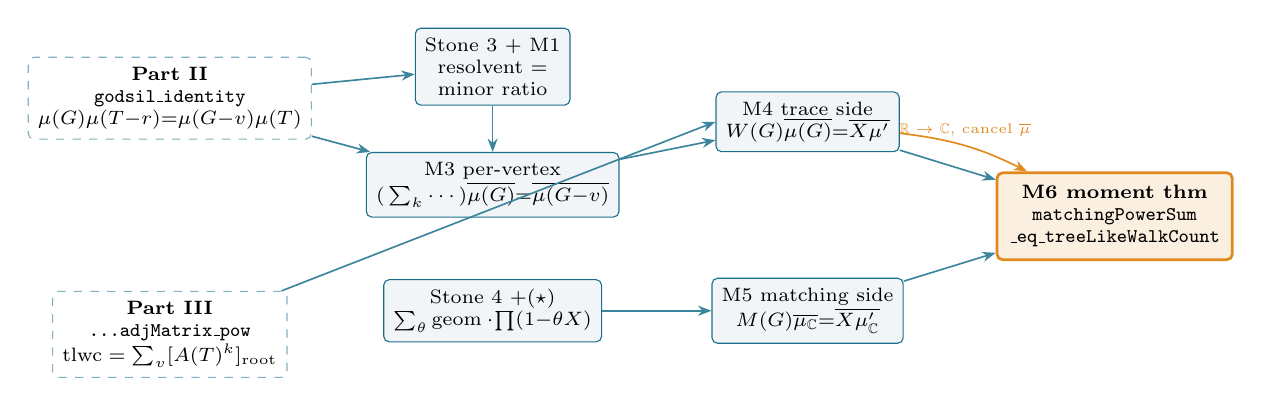
\begin{tikzpicture}[
  font=\scriptsize,
  node distance=4.5mm,
  ext/.style={draw=ggteal!55,dashed,rounded corners=2pt,fill=white,inner sep=3.5pt,align=center},
  st/.style={draw=ggteal,rounded corners=2pt,fill=ggband!40,inner sep=3.5pt,align=center},
  goal/.style={draw=ggamber,line width=1pt,rounded corners=2pt,fill=ggamber!14,inner sep=4.5pt,align=center},
  fl/.style={-{Stealth[length=1.7mm]},ggteal!85,semithick}]
% external inputs
\node[ext] (p2) at (0,1.5) {\textbf{Part~II}\\ \lean{godsil\_identity}\\ $\mu(G)\mu(T{-}r){=}\mu(G{-}v)\mu(T)$};
\node[ext] (p3) at (0,-1.5) {\textbf{Part~III}\\ \lean{...adjMatrix\_pow}\\ $\mathrm{tlwc}=\sum_v[A(T)^k]_{\rm root}$};
% trace column
\node[st] (s3) at (4.1,1.9) {Stone 3 $+$ M1\\ resolvent $=$\\ minor ratio};
\node[st] (m3) at (4.1,0.4) {M3 per-vertex\\ $(\,\sum_k\cdots)\overline{\mu(G)}{=}\overline{\mu(G{-}v)}$};
\node[st] (m4) at (8.1,1.2) {M4 trace side\\ $W(G)\overline{\mu(G)}{=}\overline{X\mu'}$};
% matching column
\node[st] (s4) at (4.1,-1.2) {Stone 4 $+(\star)$\\ $\sum_\theta\mathrm{geom}\cdot\!\prod(1{-}\theta X)$};
\node[st] (m5) at (8.1,-1.2) {M5 matching side\\ $M(G)\overline{\mu_\C}{=}\overline{X\mu_\C'}$};
% goal
\node[goal] (thm) at (12.0,0) {\textbf{M6 moment thm}\\ \lean{matchingPowerSum}\\ \lean{\_eq\_treeLikeWalkCount}};
\draw[fl] (p2) -- (s3); \draw[fl] (p2) -- (m3);
\draw[fl] (p3) -- (m4.west);
\draw[fl] (s3) -- (m3); \draw[fl] (m3) -- (m4);
\draw[fl] (s4) -- (m5);
\draw[fl] (m4) -- (thm); \draw[fl] (m5) -- (thm);
\draw[fl,ggamber] (m4) to[bend left=10] node[above,font=\tiny,text=ggamber]{$\R\to\C$, cancel $\overline{\mu}$} (thm);
\end{tikzpicture}
\caption{Formal-dependency roadmap. Two external inputs (Parts~II and~III, dashed) feed a trace
column and a matching column; each terminates at the same reflected derivative $\overline{X\mu'}$
(M4 over $\R$, M5 over $\C$); the base change $\R\to\C$ and cancellation of the unit $\overline{\mu}$
close the moment theorem (M6, amber). Every box is a \lean{sorry}-free Lean result; cf.\
Table~\ref{tab:results}.}
\label{fig:roadmap}
\end{figure}

% ---------------------------------------------------------------
\section{The two generating functions}
\label{sec:objects}

\emph{What are the two objects, and in which ring do they meet?} Keeping them honestly apart matters,
because the whole content is that they coincide. The trace side is a count of natural numbers; the
matching side lives over $\C$, because the roots do.

The trace side is the formal power series whose $k$-th coefficient is the tree-like walk count,
\[
  W(G)\;:=\;\mathrm{mk}\bigl(k\mapsto(\mathrm{treeLikeWalkCount}(G,k):\R)\bigr)\ \in\ \R\llbracket X\rrbracket .
\]
By Part~III's spectral form it is a sum of root--root resolvents of the path trees; we will keep it
over $\R$ as long as possible and cross to $\C$ only at the end. The matching side is
\[
  M(G)\;:=\;\mathrm{mk}\bigl(k\mapsto p_k(G)\bigr)\ \in\ \C\llbracket X\rrbracket,
  \qquad p_k(G)=\sum_{\theta\in\mathrm{roots}(\mu_\C)}\theta^{k},
\]
where $\mu_\C:=\mu(G)$ mapped along $\R\hookrightarrow\C$, so that its multiset of roots has exactly
$n=|V(G)|$ elements (\lean{matchingPowerSum}, \lean{matchingPowerSum\_genfun}). The proof equates the
images of $W(G)$ and $M(G)$ in $\C\llbracket X\rrbracket$.

Throughout, $\overline{p}$ denotes the coercion of the reversed polynomial $\rev(p)=\reflect_{\deg
p}(p)$ into a power-series ring, and $\reflect_N$ is the degree-$N$ reflection
$x^j\mapsto x^{N-j}$. The single algebraic fact we lean on repeatedly is that $\reflect_N$ is
additive in $p$ at a \emph{fixed} length $N$, even though $\rev$ (which reflects at each polynomial's
own degree) is not.

% ---------------------------------------------------------------
\section{The trace side becomes a reversed matching polynomial}
\label{sec:trace}

\emph{Part~III left the trace side as a sum of matrix powers of trees. How does a sum over path
trees, each a different forest, become a statement about $G$'s own matching polynomial?} Through three
moves: a determinant collapse that identifies the resolvent's numerator, Part~II's divisibility
identity that trades the tree for the graph, and a reflection that sums the pieces. The walk
generating function of a graph is itself a classical object~\cite{GodsilMoments}; what is new is the
machine-checked path from it to the matching polynomial.

\paragraph{The per-tree resolvent.} For any matrix $M$ over a commutative ring and index $i$, the
diagonal of the resolvent generates the diagonal matrix powers,
\[
  \Bigl(\sum_{k\ge0}[M^k]_{ii}X^k\Bigr)\cdot\overline{\charpolyRev(M)}
  \;=\;\overline{\charpolyRev\bigl(M\!\restriction_{j\neq i}\bigr)},
\]
the single-entry case of Cramer's rule, where $\charpolyRev(M)=\det(1-XM)$ is the reversed
characteristic polynomial (\lean{resolventGenfun\_diag\_mul\_coe\_charpolyRev}). Its proof needed one
general lemma absent from Mathlib: the principal-minor identity
$\mathrm{adj}(M)_{ii}=\det(M\!\restriction_{j\neq i})$ over an arbitrary finite index type, which we
prove by a block-triangular reindexing $n\simeq\{i\}\sqcup\{j\neq i\}$ rather than the \lean{Fin}-only
cofactor expansion Mathlib carries (\lean{adjugate\_diag\_eq\_det\_submatrix\_ne}).

\paragraph{From the submatrix to the isolated root.} Part~III's spectral form deletes the root as a
matrix \emph{index}; Part~II's divisibility identity speaks of deleting its \emph{edges}. The two
must be reconciled. Deleting all edges at the root $r$ of $T=T(G,v)$ leaves a zero row, so
$1-X\,A(T_{\widehat r})$ has its $r$-th row equal to the basis vector $e_r$, and its determinant
collapses to the $\{j\neq r\}$ minor---which is exactly the submatrix the resolvent produced. Hence
\keyeq{\overline{\charpolyRev\bigl(A(T_{\widehat r})\bigr)}\;=\;\overline{\charpolyRev\bigl(A(T)\!\restriction_{j\neq
r}\bigr)},}
the bridge between the two deletions (\lean{coe\_charpolyRev\_adjMatrix\_deleteIncidenceSet}, resting
on the general \lean{det\_eq\_det\_submatrix\_ne\_of\_row\_eq\_single}).

\paragraph{The per-vertex identity.} Now Part~II enters. Reversing the divisibility identity
$\mu(G)\,\mu(T_{\widehat r})=\mu(G-v)\,\mu(T)$ over the integral domain $\R[X]$ (reversal is
multiplicative there, and $\rev\circ\det=\charpolyRev$), the forest bridge $\mu(T)=\det(xI-A(T))$
turns each reversed matching polynomial into a $\charpolyRev$; cancelling the common unit factor
$\overline{\charpolyRev(A(T))}$ collapses the whole per-tree story to a single clean statement about
$G$:
\keyeq{\Bigl(\sum_k[A(T(G,v))^k]_{\mathrm{root}}X^k\Bigr)\cdot\overline{\mu(G)}\;=\;\overline{\mu(G-v)} }
(\lean{resolventGenfun\_pathTree\_mul\_reverse\_matchingPoly}; here $G-v$ is the incidence-deletion
form, isolating $v$). The path tree has done its work and vanished: only $\mu(G)$ and $\mu(G-v)$
remain.

\paragraph{Summing over $v$.} Summing the per-vertex identity over all vertices, the left side becomes
$W(G)\cdot\overline{\mu(G)}$ (Part~III's spectral form, with an $\N\to\R$ cast supplied by
\lean{Matrix.map\_pow}). The right side is $\sum_v\overline{\mu(G-v)}$, and here the reflection
bookkeeping pays off: every $\mu(G-v)$ has the same degree $n$, so the reversals share a length and
$\sum_v\rev(\mu(G-v))=\reflect_n(\sum_v\mu(G-v))$ (\lean{sum\_reverse\_eq\_reflect\_sum}). The
vertex-deletion derivative law $\sum_v\mu(G-v)=X\,\mu'(G)$ (\lean{sum\_matchingPoly\_deleteIncidenceSet},
proved in the companion to Part~II) finishes the move:
\keyeq{W(G)\cdot\overline{\mu(G)}\;=\;\overline{X\,\mu'(G)}.}
{\sloppy The entire trace side is now one reflected matching polynomial
(\lean{mk\_treeLikeWalkCount\_mul\_reverse\_eq}). Using $\reflect_n$, rather than $\rev$, for the
numerator is what lets us avoid ever computing the degree of $X\mu'$.\par}

% ---------------------------------------------------------------
\section{The matching side becomes the same}
\label{sec:match}

\emph{The matching side knows nothing of trees; it knows only the roots. How does the generating
function of $\sum_i\theta_i^k$ become the very same $\overline{X\mu'}$?} Through a geometric series
that cancels a product, and the classical fact that a polynomial's derivative is the sum of its
leave-one-out factor products.

\paragraph{Power sums as geometric series.} The generating function of the power sums is, coefficient
by coefficient, the multiset-sum of per-root geometric series,
\[
  M(G)\;=\;\sum_{\theta}\mathrm{geomSeries}(\theta),\qquad
  \mathrm{geomSeries}(\theta)=\sum_k\theta^kX^k=(1-\theta X)^{-1}
\]
(\lean{powerSum\_genfun}). Multiplying by the reversed factor product collapses it, root by root: since
$\mathrm{geomSeries}(\theta)\,(1-\theta X)=1$ and the whole product
$\prod_\theta(1-\theta X)$ factors as $(1-\theta X)$ times the leave-one-out product, one obtains
\keyeq{\Bigl(\sum_\theta\mathrm{geomSeries}(\theta)\Bigr)\cdot\!\prod_\theta(1-\theta X)\;=\;\sum_\theta\!\prod_{\varphi\neq\theta}(1-\varphi X)}
with \emph{no} derivative and \emph{no} Newton recursion---only the cancellation of one factor
(\lean{geomSeries\_sum\_mul\_prod}). Because $\mu_\C$ is monic and splits over $\C$, it equals
$\prod_\theta(X-\theta)$, and reversal sends this to $\prod_\theta(1-\theta X)$
(\lean{reverse\_prod\_X\_sub\_C}); so the left factor is $\overline{\mu_\C}$.

\paragraph{The leave-one-out sum is the reflected derivative.} The right-hand side is the matching
mirror of the trace side's numerator. Classically, for a split polynomial,
$\mu_\C'=\sum_\theta\prod_{\varphi\neq\theta}(X-\varphi)$ (\lean{derivative\_prod\_X\_sub\_C}, the
product rule). Each leave-one-out product has degree $n-1$, so $X\cdot\prod_{\varphi\neq\theta}(X-\varphi)$
has degree $n$; reflecting at the fixed length $n$ and using $\rev(Xq)=\rev(q)$ termwise,
\keyeq{\sum_\theta\prod_{\varphi\neq\theta}(1-\varphi X)\;=\;\reflect_n\!\bigl(X\,\mu_\C'\bigr)}
(\lean{reflect\_X\_mul\_derivative\_eq\_sum\_prod}). Chaining the two boxes through the
power-series coercion of a product and a sum gives the matching analogue of the trace identity,
\keyeq{M(G)\cdot\overline{\mu_\C}\;=\;\overline{X\,\mu_\C'}}
(\lean{mk\_powerSum\_mul\_reverse}, specialized to $\mu_\C$ in
\lean{mk\_matchingPowerSum\_mul\_reverse\_eq}). Both sides now speak the same reflected polynomial.

% ---------------------------------------------------------------
\section{The weld}
\label{sec:weld}

\emph{Two identities, one over $\R$ and one over $\C$, both ending at $\overline{X\mu'}$. What is left
but to put them together?} A change of base and a cancellation.

The trace identity lives over $\R$; the matching one over $\C$. Mapping the former along the ring
homomorphism $\R\to\C$ commutes with everything in sight---with $\mathrm{mk}$ (through
\lean{coeff\_map} and $\N$-casts), with the polynomial-to-series coercion, with $\rev$ (which is
$\reflect$ at a degree preserved by an injective map), with $\reflect$, and with the derivative
(\lean{reflect\_map}, \lean{derivative\_map}, \lean{natDegree\_map\_eq\_of\_injective}). The image of
the trace identity is therefore
\[
  W_\C(G)\cdot\overline{\mu_\C}\;=\;\overline{X\,\mu_\C'},
  \qquad W_\C(G)=\mathrm{mk}\bigl(k\mapsto(\mathrm{treeLikeWalkCount}(G,k):\C)\bigr),
\]
identical in its right-hand side to the matching identity $M(G)\cdot\overline{\mu_\C}=\overline{X\mu_\C'}$.
Hence $W_\C(G)\cdot\overline{\mu_\C}=M(G)\cdot\overline{\mu_\C}$. The reversed matching polynomial
$\overline{\mu_\C}$ is a unit: $\mu_\C$ is monic, so $\rev(\mu_\C)$ has constant term $1$ and is
nonzero, and $\C\llbracket X\rrbracket$ is an integral domain. Cancelling it gives
$W_\C(G)=M(G)$, and reading the coefficient of $X^k$ is the theorem.

\begin{theorem}[Godsil's moment theorem, machine-checked]
\label{thm:moment}
For every finite graph $G$ on the vertex type $V$, every $k\in\N$,
\[
  p_k(G)\;=\;\sum_{\theta\in\mathrm{roots}(\mu_\C)}\theta^{\,k}\;=\;\bigl(\mathrm{treeLikeWalkCount}(G,k):\C\bigr).
\]
In Lean: \lean{matchingPowerSum\_eq\_treeLikeWalkCount}. The proof is \lean{sorry}-free and depends
only on \lean{propext}, \lean{Classical.choice}, \lean{Quot.sound}.
\end{theorem}

\begin{figure}[t]
\centering
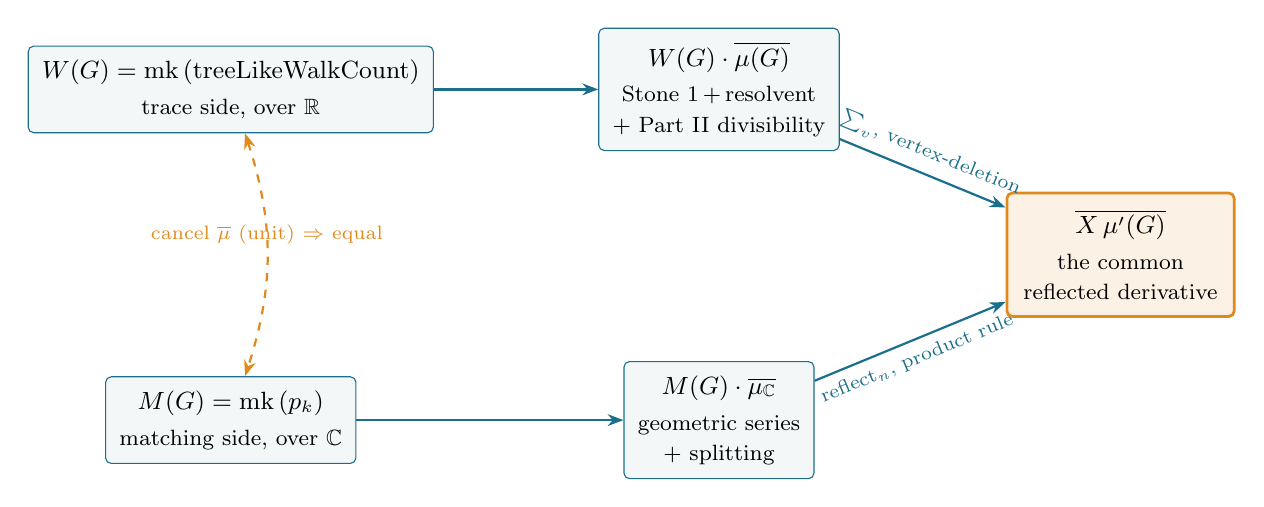
\begin{tikzpicture}[
  font=\small,
  box/.style={draw=ggteal,rounded corners=2pt,fill=ggband!35,inner sep=5pt,align=center},
  meet/.style={draw=ggamber,line width=1pt,rounded corners=2pt,fill=ggamber!12,inner sep=6pt,align=center},
  ar/.style={-{Stealth[length=2mm]},ggteal,thick}]
\node[box] (w) at (0,2.1) {$W(G)=\mathrm{mk}\,(\mathrm{treeLikeWalkCount})$\\[2pt]\footnotesize trace side, over $\R$};
\node[box] (m) at (0,-2.1) {$M(G)=\mathrm{mk}\,(p_k)$\\[2pt]\footnotesize matching side, over $\C$};
\node[box] (wt) at (6.2,2.1) {$W(G)\cdot\overline{\mu(G)}$\\[2pt]\footnotesize Stone 1\,$+$\,resolvent\\\footnotesize $+$ Part~II divisibility};
\node[box] (mt) at (6.2,-2.1) {$M(G)\cdot\overline{\mu_\C}$\\[2pt]\footnotesize geometric series\\\footnotesize $+$ splitting};
\node[meet] (mid) at (11.3,0) {$\overline{X\,\mu'(G)}$\\[2pt]\footnotesize the common\\\footnotesize reflected derivative};
\draw[ar] (w) -- (wt);
\draw[ar] (m) -- (mt);
\draw[ar] (wt) -- node[above,sloped,font=\scriptsize]{$\sum_v$, vertex-deletion} (mid);
\draw[ar] (mt) -- node[below,sloped,font=\scriptsize]{$\reflect_n$, product rule} (mid);
\draw[{Stealth[length=2mm]}-{Stealth[length=2mm]},ggamber,thick,dashed]
  (w) to[bend left=18] node[above,font=\scriptsize,text=ggamber]{cancel $\overline{\mu}$ (unit) $\Rightarrow$ equal} (m);
\end{tikzpicture}
\caption{The weld. Both generating functions, multiplied by the reversed matching polynomial, are
forced to equal the same reflected derivative $\overline{X\mu'(G)}$ (over $\R$ on top, over $\C$
below, joined by the base change $\R\to\C$). Cancelling the unit $\overline{\mu}$ identifies the two
series; the coefficient of $X^k$ is the moment theorem.}
\label{fig:weld}
\end{figure}

% ---------------------------------------------------------------
\section{Numerical verification}
\label{sec:numeric}

\emph{A formal proof certifies the implication; what certifies that the statement formalized is the
one intended?} Every identity in this paper was de-risked numerically before any formal effort,
against exact arithmetic, and the same checks fix the theorem's two sides side by side. It is worth
seeing the theorem land on one small graph in full.

\paragraph{A worked example: the pentagon $C_5$.} Take the $5$-cycle. Its matchings are the empty one,
the five single edges, and the five pairs of non-adjacent edges, so $m_0=1,\,m_1=5,\,m_2=5$ and
\[
  \mu(C_5,x)\;=\;x^5-5x^3+5x\;=\;x\Bigl(x^2-\tfrac{5+\sqrt5}{2}\Bigr)\Bigl(x^2-\tfrac{5-\sqrt5}{2}\Bigr),
\]
with roots $\theta\in\bigl\{0,\ \pm\sqrt{(5+\sqrt5)/2},\ \pm\sqrt{(5-\sqrt5)/2}\bigr\}$. The
\emph{matching} side reads the power sums off these roots:
\[
  p_2=\sum_i\theta_i^2=\tfrac{5+\sqrt5}{2}\cdot2+\tfrac{5-\sqrt5}{2}\cdot2=10,
  \qquad
  p_4=\sum_i\theta_i^4=\Bigl(\tfrac{5+\sqrt5}{2}\Bigr)^{\!2}\!\cdot2+\Bigl(\tfrac{5-\sqrt5}{2}\Bigr)^{\!2}\!\cdot2=30.
\]
The \emph{tree-like} side counts walks. For $k=2$, a closed tree-like walk at a vertex steps to a
neighbour and back; each of the $5$ vertices has $2$ neighbours, giving $2\cdot5=10=p_2$. For $k=4$,
the girth of $C_5$ is $5$, so \emph{every} closed walk of length $4$ is tree-like (none can yet
enclose the pentagon), and the count is $\tr(A^4)=2^4+2\bigl(\tfrac{\sqrt5-1}{2}\bigr)^4+2\bigl(\tfrac{\sqrt5+1}{2}\bigr)^4=30=p_4$,
using the adjacency eigenvalues $2,\ \tfrac{\sqrt5-1}{2}\,(\times2),\ -\tfrac{\sqrt5+1}{2}\,(\times2)$.
The two sides agree, as Theorem~\ref{thm:moment} requires. The first \emph{disagreement} is the
theorem's other content: at $k=5=\mathrm{girth}$, $p_5=0$ (the polynomial is odd) while
$\tr(A^5)=10$, so the gap is $10=2\cdot5\cdot1$---the single pentagon, traversed from $5$ basepoints in
$2$ orientations. The $5$-cycle is exactly the walk that is closed but not tree-like, and it appears,
on the nose, at length $5$.

Figure~\ref{fig:traceformula} plots the two sides of the trace formula on $K_4$ and the Petersen
graph: the tree side $p_k=\sum_i\theta_i^k=\mathrm{treeLikeWalkCount}(G,k)$ (the content of
Theorem~\ref{thm:moment}) against the cycle side $\tr(A^k)$, the count of \emph{all} closed walks.
Below the girth every closed walk is tree-like, so the curves coincide; the first gap appears exactly
at $k=\mathrm{girth}$ and equals $2g\,c_g$, twice the girth times the number of shortest cycles---$24$
on $K_4$ ($g=3$, $c_3=4$), $120$ on Petersen ($g=5$, $c_5=12$). Table~\ref{tab:verify} records the
matching power sums, computed from the roots of the matching polynomial, on a wider sample; in each
case they agree with the path-tree walk count of Part~III and with the girth-gap law. The matching
polynomials themselves were checked in exact $\overline{\mathbb{Q}}$ arithmetic (\texttt{SageMath});
the underlying generating-function identities (the geometric-series cancellation $(\star)$, the
reversed log-derivative $\sum_kp_kz^k=n-z\,q'/q$, and the reverse-algebra of the assembly) were each
confirmed to exact equality before the corresponding Lean lemma was written.

\begin{figure}[t]
  \centering
  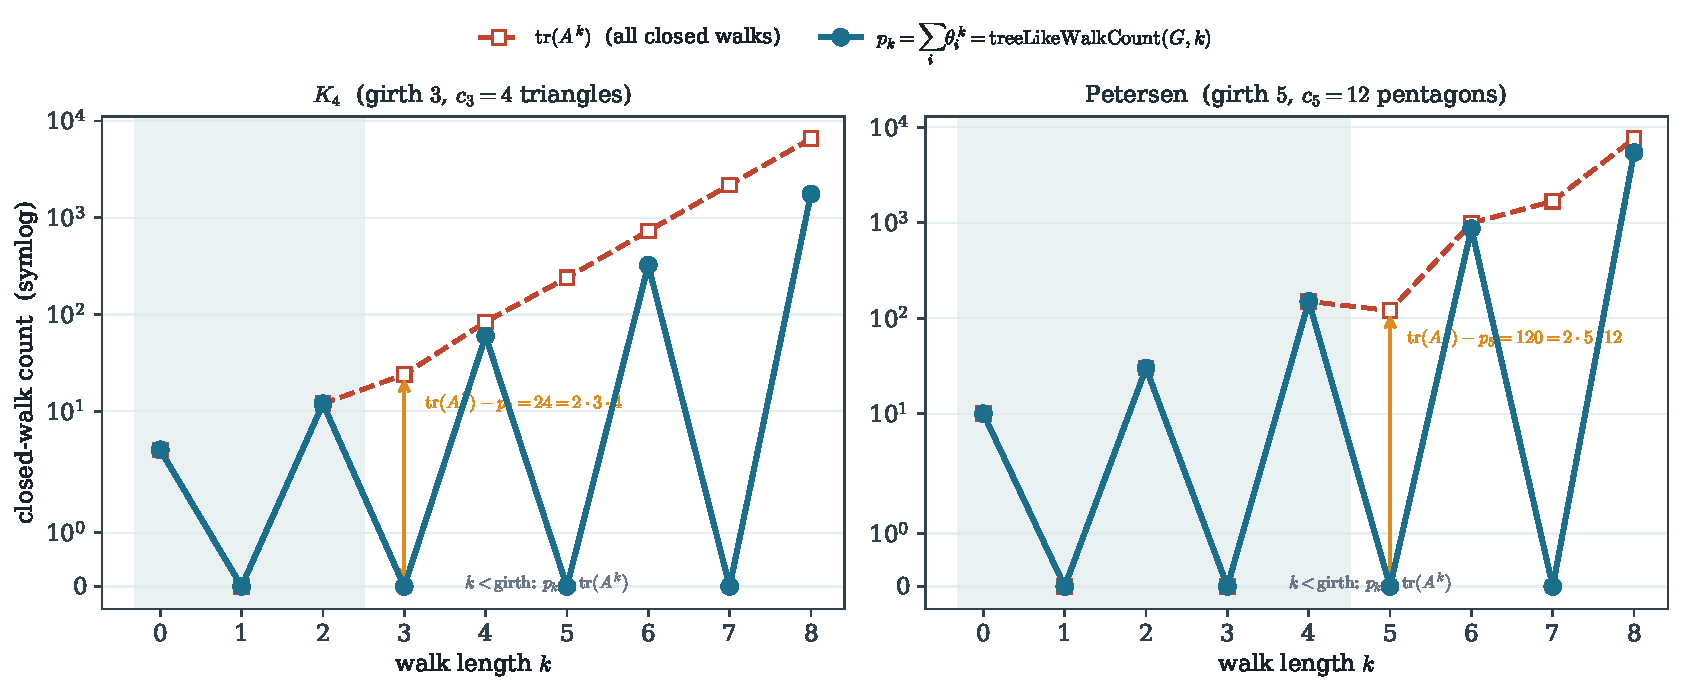
\includegraphics[width=0.98\textwidth]{figures/mt_fig1_traceformula.pdf}
  \caption{The moment theorem as the tree side of the trace formula. For $K_4$ (girth $3$) and the
  Petersen graph (girth $5$), the matching power sums $p_k=\sum_i\theta_i^{\,k}$ (teal), which
  Theorem~\ref{thm:moment} certifies equal to the tree-like walk count
  $\mathrm{treeLikeWalkCount}(G,k)=\sum_v[A(T(G,v))^k]_{\mathrm{root}}$, against $\tr(A^k)$ (red), the
  number of all closed walks. The two coincide below the girth (shaded); the first gap,
  $\tr(A^g)-p_g=2g\,c_g$, counts the shortest cycles ($g$ basepoints $\times\,2$ orientations $\times\,
  c_g$ cycles). Odd power sums vanish because the matching polynomial is even. The cycle side is the
  \emph{Bass} companion of this series; the tree side is this paper.}
  \label{fig:traceformula}
\end{figure}

\begin{table}[t]
\centering\small
\caption{Matching power sums $p_k=\sum_i\theta_i^{\,k}$, computed from the roots of $\mu(G)$ in exact
$\overline{\mathbb{Q}}$ arithmetic, equal the path-tree walk count $\mathrm{treeLikeWalkCount}(G,k)$
of Part~III for every $G$ and $k$ (the content of Theorem~\ref{thm:moment}). Odd $p_k$ vanish. The
final column is the first trace-formula gap $\tr(A^{g})-p_{g}$ at $k=\mathrm{girth}\;g$, matching the
shortest-cycle law $2g\,c_g$.}
\label{tab:verify}
\rowcolors{2}{ggband!30}{white}
\begin{tabular}{@{}lccccccc@{}}
\toprule
\rowcolor{ggteal}
{\color{white}\textbf{$G$}} & {\color{white}$n$} & {\color{white}girth} &
{\color{white}$p_0$} & {\color{white}$p_2$} & {\color{white}$p_4$} & {\color{white}$p_6$} &
{\color{white}$\tr(A^{g})-p_{g}=2g\,c_g$}\\
\midrule
$K_4$        & $4$  & $3$ & $4$  & $12$ & $60$  & $324$  & $24=2\cdot3\cdot4$\\
$C_5$        & $5$  & $5$ & $5$  & $10$ & $30$  & $100$  & $10=2\cdot5\cdot1$\\
$K_{3,3}$    & $6$  & $4$ & $6$  & $18$ & $90$  & $522$  & $72=2\cdot4\cdot9$\\
Petersen     & $10$ & $5$ & $10$ & $30$ & $150$ & $870$  & $120=2\cdot5\cdot12$\\
\bottomrule
\end{tabular}
\end{table}

% ---------------------------------------------------------------
\section{The boundary, now closed---and the route the prequel did not predict}
\label{sec:boundary}

\emph{Part~III mapped this completion as ``the single-entry resolvent identity and the univariate
Newton step.'' The resolvent step is here as foreseen. The Newton step is not---and its absence is the
one mathematically interesting thing about the proof.}

Part~III's boundary section sketched a five-link chain to the moment theorem: the resolvent identity,
the principal-minor lemma, the forest bridge, the divisibility identity, the vertex-deletion law, and
then a \emph{univariate Newton identity} equating the logarithmic derivative $\mu'/\mu$ with $\sum_k
p_kX^k$. Four of those links are exactly what Sections~\ref{sec:trace}--\ref{sec:weld} use. The fifth
is not. There is no Newton recursion in the formalization, and no univariate-root Newton lemma was
added to Mathlib's staging.

What replaced it is the cancellation of Section~\ref{sec:match}: the generating function
$\sum_\theta(1-\theta X)^{-1}$ multiplied by $\prod_\theta(1-\theta X)$ telescopes, by one factor's
worth of cancellation, into the leave-one-out sum $\sum_\theta\prod_{\varphi\neq\theta}(1-\varphi X)$,
which the product rule and a reflection identify with $\overline{X\mu'}$. Newton's identities relate
power sums to elementary symmetric functions through a recursion; here the same content appears as a
single multiset cancellation, with the derivative supplied by the product rule rather than by a
recursion on $p_k$. The logarithmic-derivative reading $\sum_kp_kX^k=n-X\,q'/q$ (with $q=\rev(\mu)$)
is still true---it was the numerical anchor that de-risked the step---but the formal proof never forms
$q'/q$; it works with cleared denominators throughout, which is why it needs no inverse and no
recursion. This is the kind of small surprise a formalization is good at surfacing: the route that
looks canonical on paper (Newton) is not the cheapest route past the machine.

The principal-minor lemma Part~III flagged as ``the one genuinely new linear-algebra lemma'' is
present (\lean{adjugate\_diag\_eq\_det\_submatrix\_ne}), and so is its determinant sibling for an
isolated row (\lean{det\_eq\_det\_submatrix\_ne\_of\_row\_eq\_single}); both are graph-free and kept in
canonical form. The reflection-of-a-sum lemma (\lean{sum\_reverse\_eq\_reflect\_sum}) and the reverse
of a split product (\lean{reverse\_prod\_X\_sub\_C}) are likewise general. Together with the cycle side
in the \emph{Bass} companion~\cite{Bass}, the finite matching/Ihara trace formula now has both of its
ends---$\tr(A^k)$ counting all closed walks and $p_k$ counting the tree-like ones---on certified
ground in one library; below the girth their coefficients coincide as theorems, and the first gap is a
count of shortest cycles, waiting to be read off.

% ---------------------------------------------------------------
\section{Implications and methodology}
\label{sec:methodology}

The formalization and manuscript were developed with AI assistance (Claude, Anthropic); the author set
the research targets, judged the mathematics, and is responsible for all claims. Every theorem named
here compiles \lean{sorry}-free against the pinned Mathlib revision~\cite{Mathlib} and depends only on
the three standard axioms, re-verifiable with \lean{\#print axioms}.

\paragraph{A false green, and the lesson banked.} One identity
(\lean{godsil\_resolvent\_charpoly\_form}) was, for a time, silently broken: an incremental
\lean{lake build} replayed a stale compiled object and reported success while the source no longer
compiled. The lesson is worth banking---a passing per-target build is not proof that a theorem
compiles; only a clean elaboration of the file is---and every identity in this paper was re-checked by
elaborating its module from source.

\paragraph{Where it applies, and how.} The moment theorem is the bridge between two ways of reading a
graph: as a combinatorial object whose walks one counts, and as the carrier of a spectrum---a ghost
one, not the graph's adjacency spectrum---whose moments one bounds. It is precisely the identity invoked, usually tacitly, wherever one of these is
estimated through the other. Concretely:
\begin{itemize}
\item \emph{Eigenvalue bounds by the method of moments.} The largest matching root obeys
$\theta_{\max}=\lim_k p_{2k}^{1/2k}$, and the moment theorem makes each $p_{2k}$ a \emph{walk count}
on the path tree---an explicitly bounded combinatorial quantity, dominated by walks on the infinite
$(\Delta-1)$-ary universal cover, whose spectral density is the Kesten--McKay
law~\cite{McKay,AngelFriedmanHoory}. This is the route to Godsil's bound
$\theta_{\max}\le2\sqrt{\Delta-1}$,
the matching analogue of the spectral-radius estimate, and the certified $p_k$ is its raw material.
\item \emph{Expander and Ramanujan thresholds.} The band edge $2\sqrt{\Delta-1}$ separating a
$\Delta$-regular graph's trivial eigenvalue from the rest is the same number; a Ramanujan graph is one
whose nontrivial spectrum stays inside it~\cite{MSS}. The moment theorem ties the matching-root
version of that threshold to a tree-like walk count, the form in which the universal-cover comparison
is cleanest.
\item \emph{Statistical mechanics.} $\mu(G,x)$ is the monomer--dimer partition function; its roots
are the zeros that control the absence of a phase transition (Heilmann--Lieb~\cite{HeilmannLieb}), and
their power sums $p_k$ are the cumulant-like moments a high-temperature expansion produces. The
theorem reads those moments off the graph's tree-like walks.
\item \emph{Networks via the non-backtracking operator.} The cycle side of the trace formula,
$\tr(A^k)$ and its non-backtracking refinement $\tr(B^k)$, governs percolation and community-detection
thresholds on networks~\cite{Hashimoto,IharaBass}; the moment theorem supplies the tree side against
which those cycle counts are measured, and the first gap, $\tr(A^g)-p_g=2g\,c_g$, is a certified
shortest-cycle count.
\end{itemize}
This paper adds no new bound and no algorithm to any of these. It places the \emph{bridge itself}---the
exact identity each of them crosses---on certified ground, in the same library where the path tree
already carries a real spectrum (Part~II) and counts tree-like walks (Part~III). The same forest now
does a third job: it makes the count \emph{equal} the spectrum. A foundation, and the closing of a
four-part arc.

\paragraph{The formalized scaffold.} Table~\ref{tab:results} lists the load-bearing results, their
Lean names, and where each is proved; the general, graph-free lemmas (marked $\ast$) are kept in
canonical form for upstreaming to Mathlib.

\begin{table}[t]
\centering\small
\caption{The load-bearing formalized results. All are \lean{sorry}-free against the pinned Mathlib
revision; $\ast$ marks the general, graph-free lemmas absent from Mathlib and kept for upstreaming.}
\label{tab:results}
\rowcolors{2}{ggband!30}{white}
\begin{tabular}{@{}>{\raggedright\arraybackslash}p{0.40\textwidth}>{\raggedright\arraybackslash}p{0.42\textwidth}c@{}}
\toprule
\rowcolor{ggteal}
{\color{white}\textbf{Lean name}} & {\color{white}\textbf{Statement}} & {\color{white}\textbf{\S}}\\
\midrule
$\ast$\,\lean{det\_eq\_det\_submatrix\_ne\_of\_row\_eq\_single} & row $i=e_i\Rightarrow\det M=\det(M\!\restriction_{\neq i})$ & \ref{sec:trace}\\
\lean{coe\_charpolyRev\_adjMatrix\_deleteIncidenceSet} & $\overline{\charpolyRev A(G_{\widehat r})}=\overline{\charpolyRev(A(G)\!\restriction_{\neq r})}$ & \ref{sec:trace}\\
\lean{resolventGenfun\_diag\_mul\_coe\_charpolyRev} & $\bigl(\sum_k[M^k]_{ii}X^k\bigr)\overline{\charpolyRev M}=\overline{\charpolyRev(M\!\restriction_{\neq i})}$ & \ref{sec:trace}\\
\lean{resolventGenfun\_pathTree\_mul\_reverse\_matchingPoly} & per-vertex: $\bigl(\sum_k[A(T)^k]_{\rm root}X^k\bigr)\overline{\mu(G)}=\overline{\mu(G-v)}$ & \ref{sec:trace}\\
$\ast$\,\lean{sum\_reverse\_eq\_reflect\_sum} & $\sum_i\rev(p_i)=\reflect_N(\sum_i p_i)$ if $\deg p_i=N$ & \ref{sec:trace}\\
\lean{mk\_treeLikeWalkCount\_mul\_reverse\_eq} & trace side: $W(G)\,\overline{\mu(G)}=\overline{X\mu'(G)}$ & \ref{sec:trace}\\
\lean{geomSeries\_sum\_mul\_prod} & $\bigl(\sum_\theta\frac{1}{1-\theta X}\bigr)\prod_\theta(1-\theta X)=\sum_\theta\prod_{\varphi\neq\theta}(1-\varphi X)$ & \ref{sec:match}\\
$\ast$\,\lean{reverse\_prod\_X\_sub\_C} & $\rev\!\prod_\theta(X-\theta)=\prod_\theta(1-\theta X)$ & \ref{sec:match}\\
\lean{reflect\_X\_mul\_derivative\_eq\_sum\_prod} & $\sum_\theta\prod_{\varphi\neq\theta}(1-\varphi X)=\reflect_n(X\mu')$ & \ref{sec:match}\\
\lean{mk\_matchingPowerSum\_mul\_reverse\_eq} & matching side: $M(G)\,\overline{\mu_\C}=\overline{X\mu_\C'}$ & \ref{sec:match}\\
\lean{matchingPowerSum\_eq\_treeLikeWalkCount} & \textbf{moment theorem:} $p_k(G)=\mathrm{treeLikeWalkCount}(G,k)$ & \ref{sec:weld}\\
\bottomrule
\end{tabular}
\end{table}

% ---------------------------------------------------------------
\section{Questions left open}
\label{sec:questions}

A formalization is also a list of the next questions, sharpened until a machine could be asked them.

\begin{itemize}
\item The proof routes around Newton's identity. Is the geometric-series cancellation
\emph{equivalent} to the univariate Newton recursion as a Mathlib lemma---i.e.\ does one give a
short proof of the other---or are they genuinely different normal forms of the same content, one
recursive and one closed?
\item Both sides were forced to equal $\overline{X\mu'}$. Can the proof be refactored so that the two
generating functions are identified \emph{before} the reflection bookkeeping, purely as ratios of
reversed polynomials, leaving $\reflect_n$ out of the cancellation entirely?
\item Below the girth the moment theorem gives $p_k=\tr(A^k)$, and the first gap at $k=\mathrm{girth}$
counts shortest cycles. Now that both sides are formal objects, can the gap
$\tr(A^k)-p_k$ be evaluated at $k=\mathrm{girth}$ inside the library, yielding the cycle-counting
correction $2\,\mathrm{girth}\cdot c_g$ as a theorem?
\item The reversed-polynomial bookkeeping ($\rev$, $\reflect_N$, the unit $\overline{\mu}$) recurs in
both the matching and the Ihara/Bass sides. Is there a single \emph{reversed generating-function}
calculus that subsumes both, so that the full trace formula $\tr(A^k)=p_k+(\text{cycle terms})$ is one
identity rather than two welded halves?
\item The principal-minor and reflection lemmas are general. Pushed upstream, would they shorten
existing Mathlib developments---resultants, companion matrices, the existing \lean{charpolyRev}
API---or are they only ever useful in the company of a path tree?
\end{itemize}

And one to keep. \emph{The matching polynomial is not the characteristic polynomial of the graph's own
adjacency matrix, yet its root power sums count walks exactly as a spectrum's would; the theorem says where those moments live---but
is the spectrum they describe a bookkeeping artefact of the path tree, or, for every purpose that
consumes its moments, as real as any matrix's?}

% ---------------------------------------------------------------
\begin{thebibliography}{99}

% --- the matching polynomial and its real-rootedness ---
\bibitem{HeilmannLieb} O.~J. Heilmann and E.~H. Lieb, \emph{Theory of monomer--dimer systems},
Comm.\ Math.\ Phys.\ \textbf{25} (1972), 190--232.
\bibitem{Farrell1979} E.~J. Farrell, \emph{An introduction to matching polynomials}, J.~Combin.\
Theory Ser.~B \textbf{27} (1979), 75--86.
\bibitem{LovaszPlummer} L.~Lov\'asz and M.~D. Plummer, \emph{Matching Theory}, North-Holland Math.\
Stud.\ \textbf{121}, Amsterdam, 1986.

% --- Godsil's path tree: matchings, walks, and the moment theorem ---
\bibitem{Godsil1981a} C.~D. Godsil, \emph{Matchings and walks in graphs}, J.~Graph Theory \textbf{5}
(1981), 285--297.
\bibitem{Godsil1981b} C.~D. Godsil and I.~Gutman, \emph{On the theory of the matching polynomial},
J.~Graph Theory \textbf{5} (1981), 137--144.
\bibitem{GodsilBook} C.~D. Godsil, \emph{Algebraic Combinatorics}, Chapman \& Hall, New York, 1993.

% --- Newton's identities, the symmetric-function ancestry ---
\bibitem{Girard} A.~Girard, \emph{Invention nouvelle en l'alg\`ebre}, Amsterdam, 1629.
\bibitem{Macdonald} I.~G. Macdonald, \emph{Symmetric Functions and Hall Polynomials}, 2nd ed.,
Oxford Univ.\ Press, 1995.

% --- universal covers, non-backtracking spectra, the matching polynomial ---
\bibitem{AngelFriedmanHoory} O.~Angel, J.~Friedman, and S.~Hoory, \emph{The non-backtracking spectrum
of the universal cover of a graph}, Trans.\ Amer.\ Math.\ Soc.\ \textbf{367} (2015), 4287--4318.
\bibitem{Spier2025} T.~J. Spier, \emph{Eigenvalues of universal covers and the matching polynomial},
preprint, 2025. \texttt{arXiv:2510.05041}.
\bibitem{McKay} B.~D. McKay, \emph{The expected eigenvalue distribution of a large regular graph},
Linear Algebra Appl.\ \textbf{40} (1981), 203--216.
\bibitem{GodsilMoments} C.~D. Godsil, \emph{Walk generating functions, Christoffel--Darboux
identities and the adjacency matrix of a graph}, Combin.\ Probab.\ Comput.\ \textbf{1} (1992),
13--25.

% --- the Ihara zeta / cycle side ---
\bibitem{Hashimoto} K.~Hashimoto, \emph{Zeta functions of finite graphs and representations of
$p$-adic groups}, in \emph{Automorphic Forms and Geometry of Arithmetic Varieties}, Adv.\ Stud.\
Pure Math.\ \textbf{15}, 1989, 211--280.
\bibitem{IharaBass} H.~Bass, \emph{The Ihara--Selberg zeta function of a tree lattice}, Internat.\
J.~Math.\ \textbf{3} (1992), 717--797.

% --- Ramanujan graphs (the band edge $2\sqrt{\Delta-1}$) ---
\bibitem{MSS} A.~Marcus, D.~A. Spielman, and N.~Srivastava, \emph{Interlacing families~I: Bipartite
Ramanujan graphs of all degrees}, Ann.\ of Math.\ \textbf{182} (2015), 307--325.

% --- this series (Lean 4 / Mathlib formalizations) ---
\bibitem{PartI} C.~Mar\'in, \emph{Random Signs into Matchings: the Godsil--Gutman estimator and
real-rootedness in Lean~4} (Part~I), 2026. Zenodo, DOI \texttt{10.5281/zenodo.20517350}.
\bibitem{PartII} C.~Mar\'in, \emph{Unfolding a Graph into a Tree: A Machine-Checked Proof of the
Heilmann--Lieb Theorem in Lean~4} (Part~II), 2026. Zenodo, DOI \texttt{10.5281/zenodo.20561832}.
\bibitem{Bass} C.~Mar\'in, \emph{Folding Edges into Vertices: A Machine-Checked Proof of Bass's
Determinant Formula for the Ihara Zeta in Lean~4}, 2026. Zenodo, DOI
\texttt{10.5281/zenodo.20573120}.
\bibitem{PartIII} C.~Mar\'in, \emph{Walks that Forget the Cycles: A Machine-Checked Bijection between
Tree-Like Walks of a Graph and Walks on Godsil's Path Tree, in Lean~4} (Part~III), 2026. Zenodo, DOI
\texttt{10.5281/zenodo.20600326}.

% --- the proof assistant ---
\bibitem{Mathlib} The mathlib Community, \emph{The Lean mathematical library}, in \emph{Proc.\ 9th
ACM SIGPLAN Int.\ Conf.\ on Certified Programs and Proofs} (CPP~2020), 367--381.

\end{thebibliography}

\end{document}
